\documentclass[12pt]{article}

\usepackage[utf8]{inputenc}
\usepackage[margin=1.0in]{geometry}
\usepackage{verbatim}
\usepackage{titlesec}
\usepackage[title,titletoc,toc]{appendix}
\usepackage{amssymb}
\usepackage{amsmath}
\usepackage{amsfonts}
\usepackage{mathtools}
\usepackage{textcomp}
\usepackage{longtable}
\usepackage{float}
\usepackage{changepage}
\usepackage{lipsum}
\usepackage{graphicx}
\usepackage{caption}
\usepackage{subcaption}
\usepackage{longtable}
\usepackage{array}
\usepackage{booktabs}
\usepackage{xcolor}
\usepackage{tikz}
\usetikzlibrary{arrows.meta}
\usetikzlibrary{calc}

\usepackage{enumitem}
\usepackage{hyperref}
\hypersetup{
    linktoc=all,
    colorlinks,
    citecolor=black,
    filecolor=black,
    linkcolor=blue,
    urlcolor=black,
    breaklinks
}


% a plane with varying y coordinate
\newcommand{\planemaina}[3]{
	(-2, #1, 2) --
	++(8, 0.3, 0) --
	++(0, -5, -8) --
	++(-8, -0.3, 0) --
	cycle;
	\node[fill=white,inner sep=2pt, anchor=east] at (-2, #1, 2) {#2};
	\node[anchor=north, black!40] at (5.8, #1+0.2, 5.5) {#3};
	}
	
\newcommand{\planemainb}[3]{
	(-2, #1, 2) --
	++(8, 0.3, 0) --
	++(0, -5, -8) --
	++(-8, -0.3, 0) --
	cycle;
	\node[fill=white,inner sep=2pt, anchor=east] at (-2, #1, 2) {#2};
	\node[anchor=north, orange!85] at (4.78, #1+0.3, 2.8) {#3};
	}

\newcommand{\planelittlea}[1]{
	(-0.2, #1, 2) --
	++(1.36, 0.126, 0) --
	++(0.24, -1.68, -2.7) --
	++(-1.45, -0.156, 0) --
	cycle;
	}
	
\newcommand{\planelittleb}[1]{
	(6.7, #1, 2) --
	++(1.1, 0, 0) --
	++(0, -1.4, -1.8) --
	++(-1.3, -0, 0) --
	cycle;
	}
	
\newcommand{\planelittlec}[1]{
	(1.9, #1, 2) --
	++(0.85, 0.026, 0) --
	++(0, -1.08, -1.8) --
	++(-0.85, -0.026, 0) --
	cycle;
	}
	

\begin{document}

\pagenumbering{gobble}% Remove page numbers (and reset to 1)
\clearpage
\thispagestyle{empty}


\begin{figure}

\begin{center}
	
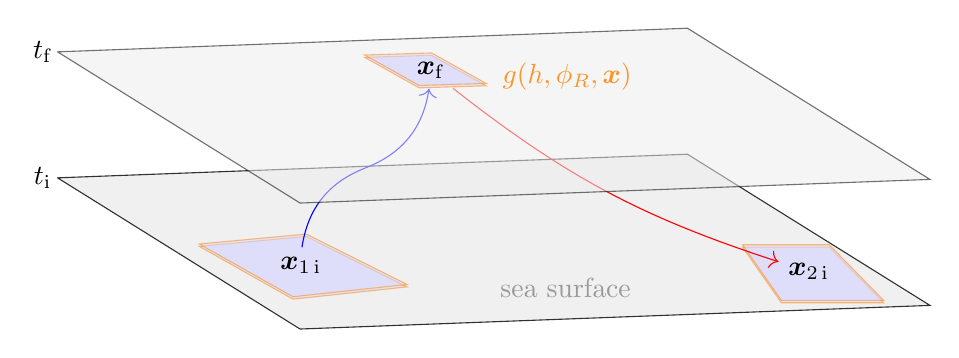
\begin{tikzpicture}

	% two planes
	\draw[fill=gray!15, opacity=0.8]\planemaina{-0.8}{$t_{\textrm{i}}$}{sea surface};
	
	\draw[orange, fill=blue!15, opacity=0.5]\planelittlea{-1.67};
	\draw[orange, fill=blue!15, opacity=0.5]\planelittlea{-1.64};
	
	\draw[orange, fill=blue!15, opacity=0.5]\planelittleb{-1.68};
	\draw[orange, fill=blue!15, opacity=0.5]\planelittleb{-1.65};
		
	\path (-0.45,-3.45,-2) node (x) {$\boldsymbol{x}_{1\,\textrm{i}}$} 
	(1,-1.17,-2.5) node (y) {$\boldsymbol{x}_{\textrm{f}}$} 
	(6,-3.53,-2) node (z) {$\boldsymbol{x}_{2\,\textrm{i}}$};
	
    \draw[-{>[scale=1.25]},blue] (x) to [bend left=30] ($(x)!0.5!(y)$) to [bend right=30] (y); 
    \draw[-{>[scale=1.25]},red] (y) to [bend right=10] (z); 
    
    %\draw[-{>[scale=1.25]},red,densely dotted] (y) to [bend left=35] ($(y)!0.3!(z)$) to [bend right=40] (z);
    %\draw[-{>[scale=1.25]},blue,densely dotted] (x) to [bend left=10] (y); 

	\draw[fill=gray!15, opacity=0.55]\planemainb{0.8}{$t_{\textrm{f}}$}{$g(h,\phi_R,\boldsymbol{x})$};
	
    \draw[orange, fill=blue!15, opacity=0.5]\planelittlec{0.73};
    \draw[orange, fill=blue!15, opacity=0.5]\planelittlec{0.76};
	
	\node at (y) {$\boldsymbol{x}_{\textrm{f}}$};

	
\end{tikzpicture}

\end{center}

\end{figure}

\end{document}
